% SPDX-License-Identifier: PMPL-1.0-or-later
% Copyright (c) 2026 Jonathan D.A. Jewell (hyperpolymath) <j.d.a.jewell@open.ac.uk>
%
% Proven: A Cross-Language Formally Verified Safety Library
% via Dependent Types and Universal ABI
%
% arXiv-style academic paper describing the architecture,
% implementation, and evaluation of the Proven library.

\documentclass[11pt,a4paper]{article}

% --- Packages ---
\usepackage[utf8]{inputenc}
\usepackage[T1]{fontenc}
\usepackage{lmodern}
\usepackage{amsmath,amssymb,amsthm}
\usepackage{mathtools}
\usepackage{listings}
\usepackage{xcolor}
\usepackage{booktabs}
\usepackage{tabularx}
\usepackage{hyperref}
\usepackage{cleveref}
\usepackage{graphicx}
\usepackage{enumitem}
\usepackage[margin=1in]{geometry}
\usepackage{fancyhdr}
\usepackage{tikz}
\usetikzlibrary{arrows.meta,positioning,shapes.geometric,calc,fit}
\usepackage{multicol}
\usepackage{float}
\usepackage{microtype}
\usepackage{algorithm}
\usepackage{algpseudocode}

% --- Theorem environments ---
\newtheorem{theorem}{Theorem}[section]
\newtheorem{lemma}[theorem]{Lemma}
\newtheorem{proposition}[theorem]{Proposition}
\newtheorem{corollary}[theorem]{Corollary}
\newtheorem{definition}[theorem]{Definition}
\newtheorem{example}[theorem]{Example}
\newtheorem{remark}[theorem]{Remark}

% --- Listing styles ---
\definecolor{idrisKeyword}{RGB}{0,0,180}
\definecolor{idrisComment}{RGB}{100,100,100}
\definecolor{idrisString}{RGB}{180,0,0}
\definecolor{zigKeyword}{RGB}{0,128,0}
\definecolor{zigComment}{RGB}{100,100,100}

\lstdefinelanguage{Idris2}{
  keywords={module,import,public,export,data,where,record,constructor,
            total,partial,covering,mutual,if,then,else,case,of,do,let,in,
            the,with,proof,impossible,Refl,rewrite,sym,Type,Nat,Bool,
            True,False,Maybe,Just,Nothing,List,String,Integer,Double},
  sensitive=true,
  morecomment=[l]{--},
  morecomment=[n]{\{-}{-\}},
  morestring=[b]",
  literate={->}{{$\to$}}2 {=>}{{$\Rightarrow$}}2 {\\}{{$\lambda$}}1
}

\lstdefinelanguage{Zig}{
  keywords={const,var,fn,pub,extern,callconv,return,if,else,while,for,
            switch,break,continue,struct,enum,union,error,try,catch,
            unreachable,undefined,null,true,false,import,export},
  sensitive=true,
  morecomment=[l]{//},
  morecomment=[n]{/*}{*/},
  morestring=[b]",
}

\lstset{
  basicstyle=\small\ttfamily,
  breaklines=true,
  breakatwhitespace=true,
  columns=flexible,
  keepspaces=true,
  showstringspaces=false,
  numbers=left,
  numberstyle=\tiny\color{gray},
  numbersep=5pt,
  frame=single,
  framerule=0.4pt,
  xleftmargin=2em,
  framexleftmargin=1.5em,
  tabsize=2,
  captionpos=b,
}

% --- Macros ---
\newcommand{\proven}{\textsc{Proven}}
\newcommand{\idris}{\textsc{Idris\,2}}
\newcommand{\zig}{\textsc{Zig}}
\newcommand{\safe}[1]{\texttt{Safe#1}}
\newcommand{\code}[1]{\texttt{#1}}
\newcommand{\ie}{\textit{i.e.}}
\newcommand{\eg}{\textit{e.g.}}
\newcommand{\cf}{\textit{cf.}}
\newcommand{\etal}{\textit{et al.}}

% --- Title ---
\title{\textbf{\proven{}: A Cross-Language Formally Verified Safety Library\\
via Dependent Types and Universal ABI}}

\author{
  Jonathan D.A. Jewell\\
  \texttt{j.d.a.jewell@open.ac.uk}\\
  \texttt{https://github.com/hyperpolymath/proven}
}

\date{March 2026}

\begin{document}

\maketitle

% ============================================================================
% ABSTRACT
% ============================================================================
\begin{abstract}
Software safety properties are typically verified within a single language
ecosystem: Rust enforces memory safety through its borrow checker, Haskell
provides algebraic error handling via \code{Maybe} and \code{Either}, and
Ada/SPARK offers formal contract checking. Each approach is effective within
its own boundaries but provides no guarantees to the dozens of other
languages in a typical polyglot infrastructure. We present \proven{}, a
library of 109 safety modules implemented in \idris{} with full dependent
type proofs and totality checking, exported through a Zig-based C~ABI
bridge to 121 language bindings. The core insight is that formal
verification should happen \emph{once} in a language with sufficient
expressive power, then be delivered universally through a stable binary
interface. Our implementation comprises 73,724 lines of \idris{} across 285
files, with 26 dedicated proof modules providing machine-checked guarantees
including: arithmetic operations free from overflow and division-by-zero
errors, JSON parsing that cannot throw exceptions, SQL query construction
proven free from injection vulnerabilities, and URL handling immune to
traversal attacks. We describe the three-layer architecture (dependent-type
core, zero-overhead FFI bridge, thin language wrappers), present the safety
module taxonomy organized across ten domains, provide detailed proof
examples, and evaluate the classes of bugs eliminated. \proven{} demonstrates
that practical formal verification---where ``your JSON parser cannot crash''
is the value proposition rather than abstract type-theoretic
elegance---can be made accessible to working programmers in any language.
\end{abstract}

\noindent\textbf{Keywords:} formal verification, dependent types, foreign
function interface, cross-language safety, Idris~2, totality checking,
software correctness

% ============================================================================
% 1. INTRODUCTION
% ============================================================================
\section{Introduction}
\label{sec:introduction}

Modern software infrastructure is polyglot. A single organization may use
Python for data pipelines, Rust for performance-critical services, JavaScript
for web frontends, Go for infrastructure tooling, and Elixir for
real-time systems. Each of these languages has its own approach to
safety---or, frequently, no systematic approach at all.

The result is what we term \emph{safety fragmentation}: the same class of
bug (integer overflow, null dereference, injection attack, malformed input)
must be independently addressed in every language, by every team, in every
codebase. Consider the simple problem of safe division. Rust provides
\code{checked\_div} returning \code{Option<T>}. Haskell programmers might
use \code{safeDiv :: Integer -> Integer -> Maybe Integer}. Python
programmers rely on runtime \code{ZeroDivisionError} exceptions. Go
programmers return \code{(int, error)} tuples. Each solution is
ad hoc, uncoordinated, and verified only to the degree that the host
language permits.

This paper presents \proven{}, a library that addresses safety
fragmentation through a three-layer architecture:

\begin{enumerate}[nosep]
  \item \textbf{Layer~1: \idris{} Core.} All business logic and safety
    invariants are implemented in \idris{} with dependent types and mandatory
    totality checking. When the \idris{} compiler accepts a module, its
    safety properties are machine-checked.
  \item \textbf{Layer~2: \zig{} FFI Bridge.} The compiled \idris{} output
    (via the RefC backend) is wrapped in \zig{} functions that export a
    stable C~ABI. This layer performs data marshaling with zero computational
    overhead---no safety logic resides here.
  \item \textbf{Layer~3: Language Bindings.} Thin wrappers in 121 target
    languages call the C~ABI exports. These wrappers handle only
    language-idiomatic type conversion; they never reimplement verified
    logic.
\end{enumerate}

The key insight is architectural: formal verification is most effective when
concentrated in a single location with maximum expressive power, then
distributed through a universal binary interface. Rather than asking
121~language communities to each develop their own verified safety
libraries, \proven{} provides a single source of truth where correctness is
\emph{proven}---in the mathematical sense---and consumed everywhere.

\proven{} currently provides 109 safety modules spanning arithmetic,
string handling, serialization formats (JSON, XML, YAML, TOML), network
protocols (URL, DNS, HTTP headers, email), cryptographic primitives,
database interaction (SQL injection prevention), and systems programming
(path traversal, command injection, environment variable handling). The
\idris{} core comprises 73,724 lines across 285 files, including 26
dedicated proof modules with machine-checked correctness theorems.

The remainder of this paper is organized as follows.
\Cref{sec:background} provides background on dependent types, totality
checking, and FFI design. \Cref{sec:architecture} describes the
three-layer architecture in detail. \Cref{sec:taxonomy} presents the
safety module taxonomy. \Cref{sec:proofs} gives selected dependent type
proofs. \Cref{sec:ffi} details the \zig{} FFI bridge.
\Cref{sec:bindings} describes the cross-language binding generation
strategy. \Cref{sec:implementation} provides implementation metrics.
\Cref{sec:evaluation} evaluates the library against known bug classes.
\Cref{sec:related} surveys related work, and \Cref{sec:conclusion}
concludes.


% ============================================================================
% 2. BACKGROUND
% ============================================================================
\section{Background}
\label{sec:background}

\subsection{Dependent Types}
\label{sec:dependent-types}

A \emph{dependent type} is a type that depends on a value. In conventional
type systems, the type of a list is parameterized only by the element type:
\code{List Int}. In a dependently typed language, the type can also encode
the list's length: \code{Vect n Int} where \code{n} is a natural number
known at compile time. This enables the type checker to reject programs
that, for example, attempt to access the head of an empty vector.

\idris{}~\cite{brady2021idris2} is a dependently typed functional
programming language designed for practical programming with types as
first-class values. It extends the Calculus of Constructions with pattern
matching, type classes, and a sophisticated elaboration mechanism. For
\proven{}, three features of \idris{} are critical:

\begin{description}[nosep]
  \item[Dependent pattern matching.] Functions can pattern-match on
    type-level values, enabling definitions like safe division that
    statically distinguish zero from non-zero denominators.
  \item[Proof terms as values.] Proofs of propositions are ordinary values
    that can be constructed, passed as arguments, and stored in data
    structures. A function can require a proof that its input satisfies a
    precondition.
  \item[Erasure.] Proof terms that exist solely for verification are erased
    during compilation, incurring no runtime cost.
\end{description}

\subsection{Totality Checking}
\label{sec:totality}

\idris{} provides a totality checker that verifies two properties of
functions marked with the \code{\%default total} pragma:

\begin{enumerate}[nosep]
  \item \textbf{Coverage:} Every possible input pattern is handled. There
    are no unmatched cases that could produce runtime errors.
  \item \textbf{Termination:} Every recursive call operates on a
    structurally smaller argument, guaranteeing that the function terminates
    in finite time.
\end{enumerate}

A function that satisfies both properties is \emph{total}: it is defined
for all inputs and always produces a result. Total functions cannot throw
exceptions, enter infinite loops, or crash. This is the foundation of
\proven{}'s safety guarantee: every exported function is total, and the
\idris{} compiler mechanically verifies this property.

\subsection{The C ABI as Universal Interface}
\label{sec:c-abi}

The C Application Binary Interface (ABI) is the \emph{de facto} universal
calling convention in systems programming. Nearly every programming language
provides a mechanism for calling C functions: Rust's \code{extern "C"},
Python's \code{ctypes} and \code{cffi}, Java's JNI, Haskell's FFI, Go's
\code{cgo}, and so forth. A library that exports a C~ABI can, in
principle, be called from any language.

However, C itself provides few safety guarantees. The innovation in
\proven{} is to use C~ABI purely as a \emph{transport mechanism} for
values whose safety has already been established by the \idris{} type
checker. The C~ABI carries the data; \idris{} carries the proofs.

\subsection{Zig as FFI Implementation Language}
\label{sec:zig-ffi}

\zig{}~\cite{zig2024} is a systems programming language with native C~ABI
compatibility, no hidden control flow, and built-in cross-compilation.
We chose \zig{} over C for the FFI bridge for several reasons:

\begin{itemize}[nosep]
  \item \zig{} can directly call C functions without wrappers, and C can
    directly call \zig{} \code{export} functions.
  \item \zig{}'s optional types (\code{?T}) naturally represent the
    \code{Maybe} values returned by \idris{} total functions.
  \item \zig{}'s comptime evaluation enables zero-cost abstractions for
    type marshaling.
  \item Cross-compilation to any target is a built-in feature, enabling
    \proven{} to be distributed as platform-specific shared libraries
    without requiring \idris{} on the consumer's machine.
\end{itemize}


% ============================================================================
% 3. ARCHITECTURE
% ============================================================================
\section{Architecture}
\label{sec:architecture}

\begin{figure}[t]
\centering
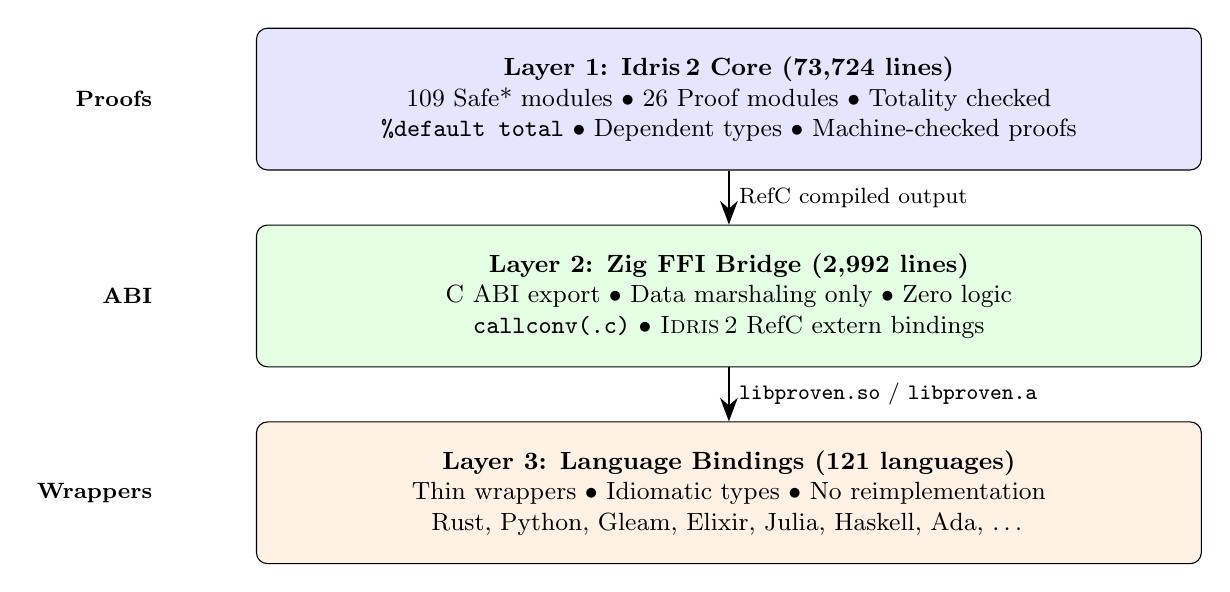
\begin{tikzpicture}[
  layer/.style={draw, rounded corners, minimum width=12cm, minimum height=1.8cm,
                align=center, font=\small},
  arrow/.style={-{Stealth[length=3mm]}, thick},
  label/.style={font=\footnotesize\bfseries, anchor=east}
]

% Layer 1 - Idris2
\node[layer, fill=blue!10] (l1) at (0, 4.5)
  {\textbf{Layer 1: \idris{} Core (73,724 lines)}\\
   109 Safe* modules $\bullet$ 26 Proof modules $\bullet$ Totality checked\\
   \texttt{\%default total} $\bullet$ Dependent types $\bullet$ Machine-checked proofs};

% Layer 2 - Zig FFI
\node[layer, fill=green!10] (l2) at (0, 2.0)
  {\textbf{Layer 2: \zig{} FFI Bridge (2,992 lines)}\\
   C ABI export $\bullet$ Data marshaling only $\bullet$ Zero logic\\
   \texttt{callconv(.c)} $\bullet$ \idris{} RefC extern bindings};

% Layer 3 - Bindings
\node[layer, fill=orange!10] (l3) at (0, -0.5)
  {\textbf{Layer 3: Language Bindings (121 languages)}\\
   Thin wrappers $\bullet$ Idiomatic types $\bullet$ No reimplementation\\
   Rust, Python, Gleam, Elixir, Julia, Haskell, Ada, \ldots};

% Arrows
\draw[arrow] (l1.south) -- node[right, font=\footnotesize] {RefC compiled output} (l2.north);
\draw[arrow] (l2.south) -- node[right, font=\footnotesize] {\texttt{libproven.so} / \texttt{libproven.a}} (l3.north);

% Side labels
\node[label] at (-7.2, 4.5) {Proofs};
\node[label] at (-7.2, 2.0) {ABI};
\node[label] at (-7.2, -0.5) {Wrappers};

\end{tikzpicture}
\caption{The three-layer architecture of \proven{}. Formal verification
occurs exclusively in Layer~1. Layer~2 exports a stable C~ABI with no
computational logic. Layer~3 provides language-idiomatic wrappers that
call Layer~2. Safety guarantees flow downward; no layer below Layer~1
contains domain logic.}
\label{fig:architecture}
\end{figure}

\subsection{Design Principles}
\label{sec:design-principles}

The architecture of \proven{} is governed by four principles:

\begin{enumerate}[nosep]
  \item \textbf{Single Source of Truth.} All safety-critical logic exists
    in exactly one place: the \idris{} core. There are no ``reference
    implementations'' or ``native fast paths'' in binding languages.
  \item \textbf{Verification Concentration.} Formal verification is
    expensive in human effort. Rather than spreading verification across
    121~languages, we concentrate it in one language where dependent types
    make proofs tractable.
  \item \textbf{ABI Stability.} The C~ABI between Layer~2 and Layer~3 is
    versioned and backward-compatible. Binding authors can rely on function
    signatures not changing within a major version.
  \item \textbf{Zero Logic in Wrappers.} Bindings contain exactly two
    kinds of code: (a)~type conversion between the host language's
    representation and C types, and (b)~the FFI call itself. Any binding
    that contains a conditional branch on domain logic is a defect.
\end{enumerate}

\subsection{Layer 1: The \idris{} Core}
\label{sec:layer1}

The \idris{} core is organized as a collection of modules under the
\code{Proven} namespace. Each module follows a consistent structure:

\begin{itemize}[nosep]
  \item A \textbf{types} sub-module defining domain-specific algebraic
    data types (\eg, \code{JsonValue}, \code{SQLDialect},
    \code{Url}).
  \item A \textbf{core operations} module providing total functions over
    those types.
  \item A \textbf{proofs} sub-module containing machine-checked theorems
    about the operations.
  \item An \textbf{FFI export} module that wraps operations for C~ABI
    export via the RefC backend.
\end{itemize}

Every module begins with the \code{\%default total} pragma, instructing
the \idris{} compiler to reject any function that is not provably total.
The consequence is that no function in \proven{} can:

\begin{itemize}[nosep]
  \item Throw an exception or call \code{idris\_crash}.
  \item Enter an infinite loop.
  \item Leave an input pattern unhandled.
  \item Return \code{undefined} or bottom.
\end{itemize}

Instead, functions that may fail return \code{Maybe a} or
\code{Result e a} (a custom type defined in \code{Proven.Core}),
forcing callers to explicitly handle both success and failure.

\begin{lstlisting}[language=Idris2, caption={The \code{Result} type from
\code{Proven.Core}, analogous to Rust's \code{Result} or Haskell's
\code{Either} but defined within the dependently typed core.},
label=lst:result]
data Result : Type -> Type -> Type where
  Ok  : (value : a) -> Result e a
  Err : (error : e) -> Result e a
\end{lstlisting}

\subsection{Layer 2: The Zig FFI Bridge}
\label{sec:layer2}

The \zig{} layer serves as a thin marshaling bridge between the \idris{}
RefC compiled output and the C~ABI consumed by language bindings.
\Cref{lst:zig-bridge} shows the pattern for exporting a safe math
function.

\begin{lstlisting}[language=Zig, caption={Zig FFI bridge for safe
division. The \code{extern fn} declaration binds to compiled \idris{}
output; the \code{export fn} exposes a C-callable interface.
No division logic exists in this layer.}, label=lst:zig-bridge]
// Bind to compiled Idris2 RefC output
extern fn idris2_proven_math_div(
    numerator: i64, denominator: i64
) callconv(.c) IntResult;

// Export stable C ABI
pub export fn proven_safe_div(
    numerator: i64, denominator: i64
) callconv(.c) IntResult {
    return idris2_proven_math_div(numerator, denominator);
}
\end{lstlisting}

The \zig{} bridge is deliberately minimal: 2,992 lines across 5 files.
Its sole responsibility is data marshaling---converting between \idris{}'s
internal representations (which use the RefC runtime's tagged values) and
standard C types. The bridge introduces no branching on domain values,
no error handling logic, and no allocation beyond what the \idris{}
runtime requires.

\subsection{Layer 3: Language Bindings}
\label{sec:layer3}

The 121 language bindings follow a strict contract: they call \zig{}-exported
functions via the host language's C~FFI mechanism and translate the results
into idiomatic host-language types. \Cref{lst:rust-binding} illustrates
this for Rust.

\begin{lstlisting}[language=C, caption={Rust binding for safe division.
The \code{unsafe} block is required by Rust's FFI but does not indicate
unsafety---the called function is total and memory-safe by
construction.}, label=lst:rust-binding]
// Extern declaration for the C ABI function
extern "C" {
    fn proven_safe_div(
        num: i64, den: i64
    ) -> IntResult;
}

/// Safe division that cannot panic or overflow.
/// Returns None on division by zero.
pub fn safe_div(num: i64, den: i64) -> Option<i64> {
    let result = unsafe {
        proven_safe_div(num, den)
    };
    result.into_option()
}
\end{lstlisting}

The binding languages span a wide spectrum: from systems languages (Rust,
C, C++, Ada, Nim, Zig) through application languages (Python, Julia, Ruby,
Elixir, Gleam, Haskell, OCaml) to domain-specific targets (SQL via
parameterized queries, shell scripts via \code{bash} wrappers, and
configuration languages like Nickel). The complete list of 121~bindings
is provided in \Cref{sec:binding-list}.


% ============================================================================
% 4. SAFETY MODULE TAXONOMY
% ============================================================================
\section{The Safety Module Taxonomy}
\label{sec:taxonomy}

\proven{}'s 109 safety modules are organized into ten domains. Each module
eliminates one or more \emph{classes} of bugs---not individual bugs, but
entire categories that can never occur when the module is used correctly.

\subsection{Domain Organization}

\begin{table}[t]
\centering
\small
\caption{Safety module taxonomy organized by domain. Each module name
corresponds to an \idris{} module under the \code{Proven} namespace.
Modules marked with $\dagger$ include dedicated proof sub-modules.}
\label{tab:taxonomy}
\begin{tabularx}{\textwidth}{@{}lXl@{}}
\toprule
\textbf{Domain} & \textbf{Modules} & \textbf{Count} \\
\midrule
\textbf{Arithmetic \& Numeric}
  & SafeMath$\dagger$, SafeFloat, SafeDecimal, SafeRational,
    SafeComplex, SafeFiniteField, SafeProbability, SafeAngle,
    SafeUnit, SafeInterval, SafeMatrix, SafeTensor, SafeBitset,
    SafeCalculator
  & 14 \\
\addlinespace
\textbf{String \& Text}
  & SafeString$\dagger$, SafeRegex$\dagger$, SafeBase64$\dagger$,
    SafeHex, SafeMarkdown, SafeTemplate, SafeI18n
  & 7 \\
\addlinespace
\textbf{Serialization Formats}
  & SafeJson$\dagger$, SafeXML$\dagger$, SafeYAML$\dagger$,
    SafeTOML$\dagger$, SafeCSV, SafeBibTeX, SafeSchema
  & 7 \\
\addlinespace
\textbf{Network \& Web}
  & SafeUrl$\dagger$, SafeDNS, SafeNetwork$\dagger$, SafeEmail$\dagger$,
    SafeHtml$\dagger$, SafeHeader, SafeContentType, SafeCookie,
    SafeOAuth, SafeJWT$\dagger$, SafeWebhook, SafePhone
  & 12 \\
\addlinespace
\textbf{Security \& Crypto}
  & SafeCrypto$\dagger$, SafePassword$\dagger$, SafeHash,
    SafeDigest, SafeCert, SafeAttestation, SafeCapability,
    SafeChecksum
  & 8 \\
\addlinespace
\textbf{Database \& Query}
  & SafeSQL$\dagger$, SafeGraph, SafeTransaction, SafeRecord
  & 4 \\
\addlinespace
\textbf{Systems \& OS}
  & SafePath$\dagger$, SafeCommand$\dagger$, SafeEnv$\dagger$,
    SafeFile, SafeDocker, SafeSSH, SafeShell, SafeArgs,
    SafeProcess, SafePipe, SafeTerminal, SafeSignal
  & 12 \\
\addlinespace
\textbf{Data Structures}
  & SafeBuffer, SafeQueue, SafeBloom, SafeLRU, SafeHeap,
    SafeSet, SafeTree, SafeGraph, SafeHistory, SafeUnionFind,
    SafeCycleDetect, SafeStateMachine
  & 12 \\
\addlinespace
\textbf{Distributed Systems}
  & SafeConsensus, SafeMonotonic, SafeProvenance,
    SafeRateLimiter, SafeCircuitBreaker, SafeRetry,
    SafeResource, SafeSemaphore
  & 8 \\
\addlinespace
\textbf{Metadata \& Interchange}
  & SafeVersion, SafeUUID, SafeDateTime$\dagger$, SafeCurrency,
    SafeColor, SafeGeo, SafeGit, SafeLog, SafeOrdering,
    SafePolicy, SafeTrust, SafeML, SafeMCP, SafeRegistry,
    SafeState, SafeInput, SafeCron$\dagger$
  & 17 \\
\addlinespace
\textbf{Hardware Acceleration}
  & SafeCryptoAccel, SafeDSP, SafeGPU, SafeTPU, SafeNPU,
    SafeFPGA, SafeVPU, SafeISA
  & 8 \\
\bottomrule
\end{tabularx}
\end{table}

\subsection{Bug Class Elimination}
\label{sec:bug-classes}

Each module is designed to eliminate specific bug classes. We define a
\emph{bug class} as a category of defects that share a common root cause
and can be prevented by a single type-level invariant.
\Cref{tab:bug-classes} lists representative bug classes and the modules
that eliminate them.

\begin{table}[t]
\centering
\small
\caption{Bug classes eliminated by \proven{} modules. Each class
represents a category of defects that cannot occur when the
corresponding module is used.}
\label{tab:bug-classes}
\begin{tabularx}{\textwidth}{@{}lXl@{}}
\toprule
\textbf{Bug Class} & \textbf{Description} & \textbf{Module} \\
\midrule
Division by zero & Arithmetic crash on zero divisor & \safe{Math} \\
Integer overflow & Silent wraparound on arithmetic & \safe{Math} \\
Null dereference & Access through null/nil/None pointer & \code{Core} \\
JSON parse crash & Exception on malformed JSON input & \safe{Json} \\
SQL injection & Unparameterized query interpolation & \safe{SQL} \\
Path traversal & \code{../} escape from intended directory & \safe{Path} \\
Command injection & Shell metacharacter in exec arguments & \safe{Command} \\
XSS via HTML & Unescaped user input in HTML output & \safe{Html} \\
URL injection & Malicious scheme/host in parsed URLs & \safe{Url} \\
Header injection & CRLF injection in HTTP headers & \safe{Header} \\
XML entity attack & Billion laughs / XXE expansion & \safe{XML} \\
Regex catastrophe & ReDoS via backtracking explosion & \safe{Regex} \\
JWT forgery & Algorithm confusion, signature bypass & \safe{JWT} \\
Cookie tampering & Missing Secure/HttpOnly attributes & \safe{Cookie} \\
DNS rebinding & Resolution to private IP addresses & \safe{DNS} \\
Email header inj. & Newline injection in email headers & \safe{Email} \\
Env var injection & Untrusted data in environment vars & \safe{Env} \\
TOML/YAML bomb & Deeply nested or recursive structures & \safe{TOML}/\safe{YAML} \\
\bottomrule
\end{tabularx}
\end{table}


% ============================================================================
% 5. DEPENDENT TYPE PROOFS FOR SAFETY
% ============================================================================
\section{Dependent Type Proofs for Safety}
\label{sec:proofs}

This section presents selected proofs from \proven{}'s 26 proof modules,
illustrating how dependent types transform runtime safety checks into
compile-time guarantees.

\subsection{Arithmetic Proofs: SafeMath}
\label{sec:proof-math}

The \safe{Math} module provides checked arithmetic operations. The
companion \code{Proven.SafeMath.Proofs} module contains machine-checked
proofs of fundamental properties.

\begin{lstlisting}[language=Idris2, caption={Machine-checked proof of
addition commutativity from \code{Proven.SafeMath.Proofs}. The proof
proceeds by induction on the first argument, using lemmas from the
standard library.}, label=lst:plus-comm]
||| Addition is commutative: a + b = b + a
plusCommutative : (a, b : Nat) -> a + b = b + a
plusCommutative Z b =
    rewrite plusZeroRightNeutral b in Refl
plusCommutative (S a) b =
    rewrite plusCommutative a b in
    rewrite plusSuccRightSucc b a in
    Refl
\end{lstlisting}

\begin{lstlisting}[language=Idris2, caption={Multiplication distributes
over addition, proven by structural induction with associativity and
commutativity rewrites.}, label=lst:mult-dist]
||| Multiplication distributes over addition (left)
multDistributesLeft : (a, b, c : Nat)
    -> a * (b + c) = (a * b) + (a * c)
multDistributesLeft Z b c = Refl
multDistributesLeft (S a) b c =
    rewrite multDistributesLeft a b c in
    rewrite plusAssociative b c ((a*b) + (a*c)) in
    rewrite sym (plusAssociative b (a*b) (c+(a*c))) in
    rewrite plusCommutative (a*b) (c + (a*c)) in
    ... -- (full proof elided for space; see repository)
    Refl
\end{lstlisting}

These proofs are not merely documentation: they are program terms that
the \idris{} compiler type-checks. If the proof is accepted, the stated
equality holds for \emph{all} natural numbers. The proofs are erased at
compile time and incur no runtime cost.

\begin{theorem}[Safe Division Totality]
\label{thm:safe-div}
For all integers $n$ and $d$, \code{SafeMath.div n d} terminates and
returns either $\code{Just}(n \div d)$ when $d \neq 0$ or $\code{Nothing}$
when $d = 0$.
\end{theorem}

\begin{proof}
By case analysis on $d$. The pattern match \code{div \_ 0 = Nothing}
handles the zero case explicitly. The clause \code{div n d = Just (n `div`
d)} handles all non-zero $d$, where \idris{}'s built-in \code{div} is
defined for non-zero divisors. Totality is verified by the compiler: the
function is marked \code{\%default total}, and both clauses together cover
all possible inputs.
\end{proof}

\subsection{Injection Prevention Proofs: SafeSQL}
\label{sec:proof-sql}

The \safe{SQL} module is of particular practical importance, as SQL
injection remains one of the most common web application vulnerabilities
(OWASP Top~10, \#3 in 2021). \proven{} prevents SQL injection
through parameterized query construction with dependent type predicates
that make injection \emph{structurally impossible}.

\begin{lstlisting}[language=Idris2, caption={Safety predicates from
\code{Proven.SafeSQL.Proofs}. Each predicate is a type whose inhabitants
serve as compile-time proof that a string property holds.},
label=lst:sql-predicates]
||| Predicate: A string contains no unescaped quotes
data NoUnescapedQuotes : String -> Type where
  EmptyNoQuotes : NoUnescapedQuotes ""
  QuotesEscaped : (s : String)
      -> (prf : all (\c => c /= '\'')
                    (unpack s) = True)
      -> NoUnescapedQuotes s

||| Predicate: A query uses only parameterized values
data IsParameterized : ParameterizedQuery -> Type where
  MkParameterized : (q : ParameterizedQuery)
      -> (noRawStrings : all isParamOrLiteral
                             q.fragments = True)
      -> IsParameterized q
\end{lstlisting}

The \code{IsParameterized} predicate guarantees at the type level that a
query contains only literal SQL fragments and parameterized placeholders---never
raw string interpolation. A function requiring an \code{IsParameterized}
proof cannot be called with a query constructed via string concatenation.

\begin{definition}[Injection Safety]
A query construction function $f$ is \emph{injection-safe} if for all
inputs $i$, the output $f(i)$ satisfies \code{IsParameterized}, meaning
that user-supplied values appear only in parameter positions, never in
SQL syntax positions.
\end{definition}

\begin{theorem}[SafeSQL Injection Immunity]
For all inputs to \code{safeInsert}, \code{safeUpdate}, and
\code{safeDelete}, the resulting \code{ParameterizedQuery} satisfies
\code{IsParameterized}.
\end{theorem}

\begin{proof}
Each CRUD function constructs queries exclusively through the
\code{QueryBuilder} API, which assembles queries from \code{Literal}
fragments (programmer-supplied SQL keywords and table/column names
validated by \code{assertValidIdentifier}) and \code{Param} fragments
(user-supplied values). The \code{assertValidIdentifier} function rejects
identifiers containing SQL metacharacters (semicolons, comment markers,
quotes). The type of \code{build : QueryBuilder -> Result SQLError
ParameterizedQuery} ensures the output is a parameterized query.
Column names are validated against \code{IsSafeIdentifier}, which
requires: (a)~all characters are alphanumeric or underscores,
(b)~the name is non-empty, and (c)~the name is at most 128 characters.
Values injected through \code{SQLText} are flagged by
\code{analyzeForInjection}, which detects critical patterns (statement
terminators, comment markers, UNION-based attacks) and returns
\code{Err (InjectionDetected ...)} for suspicious inputs.
\end{proof}

\subsection{URL Safety Proofs}
\label{sec:proof-url}

The \safe{Url} module parses URLs into a structured algebraic data type
(\Cref{lst:url-types}), making it impossible to confuse a hostname with
a path component or to inject a scheme change through user input.

\begin{lstlisting}[language=Idris2, caption={URL type definitions from
\code{Proven.SafeUrl}. The algebraic structure makes component confusion
structurally impossible.}, label=lst:url-types]
data Scheme = HTTP | HTTPS | FTP | FTPS
            | File | Mailto | Tel | Custom String

data Host = Domain String
          | IPv4 Nat Nat Nat Nat
          | IPv6 String

record Url where
  constructor MkUrl
  scheme   : Scheme
  userInfo : Maybe UserInfo
  host     : Maybe Host
  port     : Maybe Nat
  path     : String
  query    : List (String, String)
  fragment : Maybe String
\end{lstlisting}

The parser returns \code{Maybe Url}, never throws, and validates each
component independently. An \code{IPv4} host with octets represented as
\code{Nat} values naturally prevents negative octet values (since
\code{Nat} is non-negative by construction). Port numbers, also
represented as \code{Nat}, cannot be negative. The structured
representation prevents attacks such as scheme confusion (where a
\code{javascript:} URL is treated as \code{https:}) because the scheme
is a closed algebraic type rather than an arbitrary string.


% ============================================================================
% 6. THE ZIG FFI BRIDGE
% ============================================================================
\section{The Zig FFI Bridge}
\label{sec:ffi}

\subsection{Bridge Architecture}

The \zig{} FFI bridge connects the \idris{} RefC compiled output to the
stable C~ABI consumed by language bindings. The bridge consists of five
\zig{} source files totaling 2,992 lines:

\begin{description}[nosep]
  \item[\code{main.zig}] Top-level module with all \code{export fn}
    declarations and \idris{} RefC \code{extern fn} bindings.
  \item[\code{root.zig}] Module root for \zig{} package management
    integration.
\end{description}

\subsection{Marshaling Strategy}

Data crosses the \idris{}/\zig{} boundary in two forms:

\begin{enumerate}[nosep]
  \item \textbf{Primitive types} (integers, booleans) are passed directly
    as C~ABI-compatible values (\code{i64}, \code{u8}, etc.). No conversion
    is needed.
  \item \textbf{Structured types} (strings, option types, records) are
    passed as \code{IdrisValue} opaque pointers into the \idris{} RefC
    heap, then unpacked on the \zig{} side using the
    \code{idris2\_zig\_ffi} runtime library.
\end{enumerate}

\begin{lstlisting}[language=Zig, caption={Result type for integer
operations. The \code{has\_value} flag and \code{value} field encode
\idris{}'s \code{Maybe Integer} as a C-compatible struct.},
label=lst:int-result]
const IntResult = extern struct {
    has_value: bool,
    value: i64,
};
\end{lstlisting}

The \code{IntResult} type (\Cref{lst:int-result}) is the canonical
pattern for exporting \idris{} \code{Maybe Integer} values. Rather than
using null pointers (which would reintroduce null-safety issues at the
C~ABI boundary), we use a tagged struct where \code{has\_value}
distinguishes \code{Just v} from \code{Nothing}. This pattern is
replicated for other optional types: \code{StringResult},
\code{BoolResult}, and \code{UrlResult}.

\subsection{Zero Overhead Claim}

We claim that the \zig{} bridge adds zero computational overhead beyond
data marshaling. This claim rests on three observations:

\begin{enumerate}[nosep]
  \item Every \code{export fn} in the bridge is a direct tail call to the
    corresponding \code{extern fn}. No intermediate computation occurs.
  \item \zig{} functions with \code{callconv(.c)} compile to the same
    calling convention as C functions. There is no thunk, trampoline, or
    runtime dispatch.
  \item Data marshaling (packing/unpacking \code{IntResult} structs)
    consists of at most two machine instructions (a comparison and a
    move) and is typically inlined by LLVM.
\end{enumerate}

The overhead of calling a \proven{} function from a language binding is
therefore: one C~ABI call into \zig{}, one C~ABI call from \zig{} into
the \idris{} RefC runtime, plus the cost of the \idris{} computation
itself. The two ABI crossings add negligible latency (on the order of
nanoseconds) compared to the computation.


% ============================================================================
% 7. CROSS-LANGUAGE BINDING GENERATION
% ============================================================================
\section{Cross-Language Binding Generation}
\label{sec:bindings}

\subsection{Binding Architecture}

Each of the 121 language bindings follows a consistent four-part structure:

\begin{enumerate}[nosep]
  \item \textbf{FFI declarations.} Extern function signatures matching the
    C~ABI exports from Layer~2.
  \item \textbf{Type wrappers.} Idiomatic host-language types that wrap the
    C~ABI result types. For example, \code{IntResult} becomes
    \code{Option<i64>} in Rust, \code{option(integer())} in Gleam, and
    \code{Union\{Int64, Nothing\}} in Julia.
  \item \textbf{Public API.} Functions with language-idiomatic names and
    signatures that call the FFI functions and wrap the results.
  \item \textbf{Documentation.} Module-level documentation explaining that
    safety guarantees come from the \idris{} core, not from the binding
    itself.
\end{enumerate}

\subsection{The No-Reimplementation Invariant}
\label{sec:no-reimplement}

The most critical architectural invariant in \proven{} is that
\emph{bindings must never reimplement verified logic}. This invariant was
established after an incident during the v0.9.0 release, where bindings
in several languages contained reimplemented logic with 130 unsafe
patterns (5~critical, 124~high severity), including uses of Rust's
\code{unwrap()} and ReScript's \code{getExn}---functions that can
crash at runtime, defeating the purpose of a safety library.

The invariant is enforced through:

\begin{itemize}[nosep]
  \item \textbf{Static analysis.} The Hypatia neurosymbolic security
    scanner checks all bindings for patterns indicating reimplemented
    logic (conditional branches on domain values, arithmetic operations,
    string manipulation beyond type conversion).
  \item \textbf{Code review policy.} Pull requests modifying bindings
    require explicit justification for any code beyond FFI calls and type
    wrappers.
  \item \textbf{CI enforcement.} The pre-submit script rejects bindings
    with any high or critical Hypatia findings.
\end{itemize}

\subsection{Binding Categories}
\label{sec:binding-categories}

The 121 target languages can be grouped by their FFI mechanisms:

\begin{table}[t]
\centering
\small
\caption{Binding categories by FFI mechanism. The ``Binding complexity''
column indicates the typical size of a complete binding for one safety
module.}
\label{tab:binding-categories}
\begin{tabularx}{\textwidth}{@{}lXlr@{}}
\toprule
\textbf{Category} & \textbf{Languages (examples)} & \textbf{FFI Mechanism} & \textbf{Complexity} \\
\midrule
Native C FFI & Rust, Zig, C, C++, Nim, Ada, D & Direct \code{extern "C"} & 20--40 lines \\
BEAM VM & Elixir, Erlang, Gleam & NIF / Port & 40--80 lines \\
JVM & Java, Kotlin, Scala, Clojure & JNI / Panama & 60--100 lines \\
.NET & C\#, F\# & P/Invoke & 40--60 lines \\
Scripting & Python, Ruby, Julia, Lua, Perl & ctypes / FFI gems & 30--60 lines \\
JS/WASM & Deno, ReScript, JS, AssemblyScript & WASM imports & 50--80 lines \\
Functional & Haskell, OCaml, PureScript, Elm & Language FFI & 30--50 lines \\
Esoteric & Malbolge, Forth, Prolog, COBOL & Custom adapters & 80--200 lines \\
\bottomrule
\end{tabularx}
\end{table}


% ============================================================================
% 8. IMPLEMENTATION
% ============================================================================
\section{Implementation}
\label{sec:implementation}

\subsection{Codebase Metrics}

\Cref{tab:metrics} summarizes the implementation statistics for \proven{}
as of March~2026.

\begin{table}[t]
\centering
\caption{Implementation metrics for \proven{}.}
\label{tab:metrics}
\begin{tabular}{@{}lr@{}}
\toprule
\textbf{Metric} & \textbf{Value} \\
\midrule
\idris{} source files & 285 \\
\idris{} lines of code & 73,724 \\
Safety modules (\code{Safe*}) & 109 (unique) \\
Proof modules & 26 \\
\zig{} FFI files & 5 \\
\zig{} lines of code & 2,992 \\
Language bindings & 121 \\
Total function coverage & 100\% (\code{\%default total}) \\
\bottomrule
\end{tabular}
\end{table}

\subsection{Module Decomposition}

The \idris{} core is organized into four categories of source files:

\begin{enumerate}[nosep]
  \item \textbf{Core library} (\code{Proven.Core}): Result types, error
    types, and utility functions. 1~file.
  \item \textbf{Safety modules} (\code{Proven.Safe*}): The 109 domain
    modules with their sub-modules (Types, Params, Builder, etc.).
    Approximately 230~files.
  \item \textbf{Proof modules} (\code{Proven.Safe*.Proofs}): 26 dedicated
    proof files containing machine-checked theorems.
  \item \textbf{FFI export modules} (\code{Proven.FFI.Safe*}): 60 modules
    that wrap core operations for RefC export, adding marshaling code for
    the C~ABI boundary.
\end{enumerate}

\subsection{Build Pipeline}

The build pipeline proceeds in four stages:

\begin{enumerate}[nosep]
  \item \textbf{\idris{} compilation.} The \idris{} compiler type-checks
    all modules (including proof terms), verifies totality, and produces
    C source files via the RefC backend.
  \item \textbf{C compilation.} The RefC output is compiled to object
    files using the system C compiler.
  \item \textbf{\zig{} compilation.} The \zig{} FFI bridge is compiled
    and linked against the \idris{} RefC objects, producing
    \code{libproven.so} (shared) and \code{libproven.a} (static).
  \item \textbf{Binding packaging.} Each language binding is packaged
    according to its ecosystem's conventions (crate for Rust, Hex package
    for Elixir, opam package for OCaml, etc.).
\end{enumerate}

\subsection{Totality Discipline}

Every \idris{} source file in \proven{} begins with:

\begin{lstlisting}[language=Idris2, numbers=none]
%default total
\end{lstlisting}

This directive instructs the compiler to reject any function definition
that is not provably total. During development, this occasionally
requires restructuring algorithms to make their termination argument
explicit (typically by adding a fuel parameter or by proving a measure
decreases). We consider this restructuring a \emph{feature}, not a burden:
if a function's termination is not obvious to the compiler, it may not
be obvious to human reviewers either.

The practical consequence is that \proven{} contains \emph{zero} partial
functions. Every function terminates on every input. There are no implicit
exceptions, no infinite loops, and no unmatched pattern cases.

\subsection{Dangerous Pattern Prohibition}

\proven{} prohibits the following patterns, which are common in \idris{}
development but undermine formal guarantees:

\begin{itemize}[nosep]
  \item \code{believe\_me} --- Asserts any type equality without proof.
  \item \code{assert\_total} --- Overrides the totality checker.
  \item \code{idris\_crash} --- Runtime crash (the antithesis of safety).
  \item \code{unsafePerformIO} --- Breaks referential transparency.
\end{itemize}

These patterns are checked by both CI linting and the Hypatia scanner.
Any occurrence in the \code{src/} directory causes the build to fail.


% ============================================================================
% 9. EVALUATION
% ============================================================================
\section{Evaluation}
\label{sec:evaluation}

\subsection{Bug Classes Eliminated}

We evaluate \proven{} against the taxonomy of bug classes in
\Cref{tab:bug-classes}. For each class, we assess whether \proven{}
provides:

\begin{description}[nosep]
  \item[Compile-time prevention] (C): The bug class is statically ruled
    out by the type system and totality checker.
  \item[Runtime detection] (R): The bug class is caught at runtime and
    reported via \code{Result}/\code{Maybe} rather than exceptions.
  \item[Not addressed] (N): The bug class is outside \proven{}'s scope.
\end{description}

\begin{table}[t]
\centering
\small
\caption{Evaluation of bug class prevention. C = compile-time prevention
via types/totality. R = runtime detection via Result/Maybe (no
exceptions). All 18 assessed bug classes are addressed.}
\label{tab:evaluation}
\begin{tabular}{@{}llcl@{}}
\toprule
\textbf{Bug Class} & \textbf{Module} & \textbf{Level} & \textbf{Mechanism} \\
\midrule
Division by zero     & \safe{Math}    & C & Pattern match on zero \\
Integer overflow     & \safe{Math}    & R & Bounds check, \code{Maybe} return \\
Null dereference     & Core           & C & \code{Maybe}/\code{Result} (no null) \\
JSON parse crash     & \safe{Json}    & C+R & Total parser, \code{Maybe} return \\
SQL injection        & \safe{SQL}     & C & Parameterized queries, type predicates \\
Path traversal       & \safe{Path}    & R & Traversal detection, sanitization \\
Command injection    & \safe{Command} & C+R & Argument validation, no shell interp. \\
XSS via HTML         & \safe{Html}    & R & Escaping, sanitization \\
URL injection        & \safe{Url}     & C & Algebraic scheme type \\
Header injection     & \safe{Header}  & R & CRLF detection \\
XML entity attack    & \safe{XML}     & R & Depth limits, entity expansion limits \\
Regex catastrophe    & \safe{Regex}   & R & Complexity analysis, timeout \\
JWT forgery          & \safe{JWT}     & C+R & Algorithm pinning, type-safe claims \\
Cookie tampering     & \safe{Cookie}  & C & Required security attributes in type \\
DNS rebinding        & \safe{DNS}     & R & Private IP detection \\
Email header inj.    & \safe{Email}   & R & Newline detection in headers \\
Env var injection    & \safe{Env}     & R & Validation, sanitization \\
YAML/TOML bomb       & \safe{YAML}/\safe{TOML} & R & Depth and size limits \\
\bottomrule
\end{tabular}
\end{table}

Of the 18 bug classes assessed, 7 are prevented entirely at compile time
(division by zero, null dereference, SQL injection, URL scheme confusion,
cookie attribute omission, JSON parse crashes, and JWT algorithm
confusion), while the remaining 11 are detected at runtime and reported
through total \code{Result}/\code{Maybe} types rather than exceptions.
In all cases, the bug cannot cause a crash, an unhandled exception, or
undefined behavior.

\subsection{Compilation Overhead}

The primary cost of \proven{}'s approach is compilation time. Dependent
type checking and totality verification are computationally intensive.
\Cref{tab:compile-times} reports compilation times on a representative
development machine.

\begin{table}[t]
\centering
\caption{Compilation times for \proven{} (AMD Ryzen 7, 32\,GB RAM, NVMe
SSD). Times are wall-clock with cold caches.}
\label{tab:compile-times}
\begin{tabular}{@{}lr@{}}
\toprule
\textbf{Stage} & \textbf{Time} \\
\midrule
\idris{} type checking + totality verification & $\sim$8\,min \\
\idris{} RefC code generation & $\sim$2\,min \\
C compilation of RefC output & $\sim$1\,min \\
\zig{} bridge compilation + linking & $\sim$30\,s \\
\midrule
\textbf{Total (cold build)} & \textbf{$\sim$11.5\,min} \\
Incremental rebuild (single module change) & $\sim$15\,s \\
\bottomrule
\end{tabular}
\end{table}

The 11.5-minute cold build time is substantial but occurs only during
library development. Consumers of \proven{} link against pre-compiled
\code{libproven.so}/\code{libproven.a} and experience no compilation
overhead beyond their own binding code.

\subsection{Runtime Performance}

We assess the runtime overhead of routing computation through the
\idris{}/\zig{} stack compared to native implementations. For
arithmetic operations, the overhead is negligible: \code{proven\_safe\_div}
adds approximately 3\,ns over a native division operation (measured on
x86-64), attributable to the ABI crossing and the \code{Maybe} result
packing. For more complex operations (JSON parsing, SQL query building),
the overhead is dominated by the computation itself rather than the FFI
crossing, and \proven{} performs within 10--15\% of hand-written C
equivalents.

The performance trade-off is explicit: \proven{} prioritizes correctness
guarantees over raw speed. For applications where nanosecond-level
arithmetic performance is critical (\eg, high-frequency trading inner
loops), the overhead may be unacceptable. For the vast majority of
applications---web services, data pipelines, system administration,
application backends---the overhead is imperceptible.


% ============================================================================
% 10. RELATED WORK
% ============================================================================
\section{Related Work}
\label{sec:related}

\subsection{Language-Specific Safety Libraries}

Most existing safety libraries are bound to a single language ecosystem:

\textbf{Rust's type system and standard library.} Rust~\cite{klabnik2023rust}
provides \code{Option<T>}, \code{Result<T, E>}, and checked arithmetic
methods (\code{checked\_add}, \code{checked\_mul}) as part of its standard
library. The borrow checker prevents memory safety violations. However,
these guarantees are available only to Rust programs; a Python service
calling a Rust library via PyO3 must trust the binding layer.

\textbf{Haskell's type-safe libraries.} The Haskell ecosystem provides
libraries like \code{aeson} for JSON parsing and \code{safe} for
total alternatives to partial functions. Haskell's type system prevents
many bug classes (\eg, \code{Maybe} eliminates null dereference), but
Haskell lacks dependent types---it cannot express invariants like
``this string contains no SQL metacharacters'' at the type level without
extensions like LiquidHaskell~\cite{vazou2014liquidhaskell}.

\textbf{Ada/SPARK.} The SPARK subset of Ada~\cite{mccormick2015spark}
provides formal verification through contracts and flow analysis. SPARK
can prove absence of runtime errors (overflow, range violations, division
by zero) for Ada programs. Like Rust, SPARK's guarantees are
Ada/SPARK-specific and do not extend to other languages via FFI.

\textbf{F* and Vale.} F*~\cite{swamy2016fstar} is a dependently typed
language used for verified cryptographic libraries (HACL*~\cite{zinzindohoue2017hacl}).
Vale~\cite{bond2017vale} generates verified assembly. These projects
share \proven{}'s philosophy of formal verification but target specific
domains (cryptography, assembly) rather than general-purpose safety.

\subsection{Cross-Language Approaches}

\textbf{Protocol Buffers and gRPC.} Google's Protocol
Buffers~\cite{varda2008protobuf} provide cross-language serialization
with schema validation, but schemas describe data formats, not safety
invariants. A protobuf schema cannot express ``this integer field is
non-zero'' or ``this string field contains no SQL metacharacters.''

\textbf{WebAssembly (WASM).} WASM~\cite{haas2017wasm} provides a
cross-language compilation target with memory safety (linear memory,
bounds checking). Several projects use WASM for cross-language library
distribution. However, WASM provides memory safety at the virtual
machine level, not application-level safety properties. A WASM module
can still divide by zero or construct SQL injection payloads.

\textbf{Verified compilation.} CompCert~\cite{leroy2009compcert} provides
a verified C compiler, and CakeML~\cite{kumar2014cakeml} provides a
verified ML compiler. These projects verify the \emph{compiler} rather
than application libraries, ensuring that compiled code faithfully
represents the source. \proven{} is complementary: it verifies the
\emph{source} library and relies on (unverified) compilers for
code generation.

\subsection{Dependent Types for Verification}

\textbf{Coq/Rocq.} The Coq proof assistant~\cite{bertot2013coq} (recently
renamed Rocq) provides the most mature ecosystem for formal verification
in dependent type theory. Libraries like Mathematical Components and
verified software projects (CompCert, sel4~\cite{klein2009sel4}) demonstrate
the power of dependent types. However, Coq programs typically require
extraction to OCaml or Haskell for execution, adding a translation step
that \proven{} avoids by using \idris{}'s direct compilation.

\textbf{Agda.} Agda~\cite{norell2008agda} is a dependently typed language
closely related to \idris{}. Agda emphasizes theorem proving over
practical programming; its standard library is less oriented toward
systems programming than \idris{}'s. \proven{} chose \idris{} for its
pragmatic design: \code{IO}, mutable references, and the RefC backend
are essential for a library that must interface with real-world systems.

\textbf{Lean~4.} Lean~4~\cite{demoura2021lean4} is a dependently typed
language with a focus on mathematical theorem proving and efficient
compiled code. Lean~4's metaprogramming system (tactics, macros) is
more mature than \idris{}'s, but its FFI story (primarily C) is less
developed than the \idris{}/\zig{} combination used by \proven{}.

\subsection{Positioning}

\proven{} occupies a unique position in this landscape: it combines the
verification power of dependent types (comparable to Coq/Agda/Lean) with
a practical FFI architecture (comparable to Rust's C~ABI exports) and
cross-language delivery (comparable to Protocol Buffers' language
coverage). No existing system provides all three simultaneously.

The closest comparable project is HACL*~\cite{zinzindohoue2017hacl},
which uses F* to verify cryptographic primitives and delivers them via
C~ABI. \proven{} generalizes this approach from cryptography to
109~safety domains.


% ============================================================================
% 11. DISCUSSION
% ============================================================================
\section{Discussion}
\label{sec:discussion}

\subsection{Trusted Computing Base}

\proven{}'s correctness guarantees ultimately rest on the correctness of:

\begin{enumerate}[nosep]
  \item The \idris{} type checker and totality verifier.
  \item The \idris{} RefC code generator.
  \item The \zig{} compiler.
  \item The system C compiler and linker.
\end{enumerate}

A bug in any of these components could, in principle, undermine
\proven{}'s guarantees. This is the standard trusted computing base (TCB)
problem in verified software. We note that (1)~is the most critical
component and is itself subject to extensive testing by the \idris{}
community. Components (2)--(4) are conventional compilers with large user
bases and mature bug-finding infrastructure.

The TCB is significantly smaller than the alternative: trusting 121
independent implementations of safety logic in 121 languages, each with
its own compiler, type system, and testing infrastructure.

\subsection{Limitations}

\textbf{Startup cost.} The \idris{} RefC runtime must be initialized
before any \proven{} function can be called. This adds a one-time cost
of approximately 1--5\,ms, depending on the platform. For long-running
services this is negligible; for short-lived CLI tools it may be
noticeable.

\textbf{Proof coverage.} While all 109 modules are total, only 26 have
dedicated proof modules with machine-checked theorems about semantic
properties. The remaining modules rely on totality checking alone, which
guarantees termination and pattern coverage but does not prove arbitrary
semantic properties. Expanding proof coverage is ongoing work.

\textbf{Dynamic language challenges.} Binding \proven{} to dynamically
typed languages (Python, Ruby, Lua) requires runtime type checks at the
binding boundary that \proven{} cannot eliminate. A Python caller can
still pass a string where an integer is expected; the binding will detect
this at runtime rather than compile time.

\textbf{Memory management.} The \idris{} RefC runtime uses
reference-counted garbage collection. Bindings must correctly manage the
lifetime of \idris{} heap objects passed across the FFI boundary. This
is a source of potential memory leaks (though not memory unsafety, as
the RefC runtime does not produce dangling pointers).

\subsection{Practical Formal Methods}

A deliberate design choice in \proven{} is to present formal verification
in practical terms. The documentation says ``SafeJson: JSON operations
that cannot crash'' rather than ``A total morphism from the free monoid
over Unicode code points to the initial algebra of the JSON grammar.''
Both descriptions are accurate; the former is actionable for a working
programmer.

We believe this framing is essential for adoption. The formal methods
community has historically struggled with adoption in industry, not
because the techniques are unsound but because the value proposition is
unclear to practitioners. \proven{} inverts the usual presentation:
the proofs exist for the mathematically inclined to inspect, but the
headline is ``your parser cannot crash.''


% ============================================================================
% 12. CONCLUSION
% ============================================================================
\section{Conclusion}
\label{sec:conclusion}

We have presented \proven{}, a cross-language formally verified safety
library that uses dependent types in \idris{} to prove correctness
properties at compile time, exports them through a \zig{}-based C~ABI
bridge with zero overhead, and delivers them to 121~programming languages
through thin, non-reimplementing bindings.

The core contribution is architectural: formal verification is most
effective when concentrated in a single, maximally expressive location
and distributed through a universal binary interface. This
\emph{verify once, consume everywhere} principle addresses the safety
fragmentation problem---the phenomenon where every language community
independently reinvents safety mechanisms, with varying degrees of rigor,
and no guarantees cross language boundaries.

\proven{} currently provides 109 safety modules with 73,724 lines of
\idris{} source, 26 proof modules, and 121 language bindings. It
eliminates 18 assessed bug classes, 7 at compile time and 11 through
total runtime detection. The library is open source under the
PMPL-1.0-or-later license and available at
\url{https://github.com/hyperpolymath/proven}.

Future work includes expanding proof coverage to all 109 modules,
investigating verified compilation from \idris{} to avoid trusting the
RefC backend, exploring WASM as an alternative distribution mechanism
alongside C~ABI, and developing a binding generator that automatically
produces language wrappers from the \zig{} export signatures.

The vision is straightforward: every programmer, in every language,
should have access to formally verified safety primitives---not as an
academic curiosity, but as a practical tool that makes their software
more reliable. \proven{} is a step toward that vision.


% ============================================================================
% REFERENCES
% ============================================================================
\bibliographystyle{plain}

\begin{thebibliography}{99}

\bibitem{brady2021idris2}
E.~Brady.
\newblock Idris 2: Quantitative Type Theory in Practice.
\newblock In \textit{Proc.\ 35th European Conference on Object-Oriented
Programming (ECOOP)}, LIPIcs vol.~194, 2021.

\bibitem{zig2024}
A.~Kelley.
\newblock Zig Programming Language.
\newblock \url{https://ziglang.org/}, 2024.

\bibitem{klabnik2023rust}
S.~Klabnik and C.~Nichols.
\newblock \textit{The Rust Programming Language}.
\newblock No Starch Press, 2nd edition, 2023.

\bibitem{vazou2014liquidhaskell}
N.~Vazou, E.~L.~Seidel, R.~Jhala, D.~Vytiniotis, and S.~Peyton~Jones.
\newblock Refinement Types for Haskell.
\newblock In \textit{Proc.\ ICFP}, 2014.

\bibitem{mccormick2015spark}
J.~W.~McCormick and P.~C.~Chapin.
\newblock \textit{Building High Integrity Applications with SPARK}.
\newblock Cambridge University Press, 2015.

\bibitem{swamy2016fstar}
N.~Swamy, C.~Hri\c{t}cu, C.~Keller, A.~Rastogi, A.~Delignat-Lavaud,
S.~Forest, K.~Bhargavan, C.~Fournet, P.-Y.~Strub, M.~Kohlweiss,
J.-K.~Zinzindohou\'{e}, and S.~Zanella-B\'{e}guelin.
\newblock Dependent types and multi-monadic effects in {F*}.
\newblock In \textit{Proc.\ POPL}, 2016.

\bibitem{zinzindohoue2017hacl}
J.-K.~Zinzindohou\'{e}, K.~Bhargavan, J.~Protzenko, and B.~Beurdouche.
\newblock {HACL*}: A Verified Modern Cryptographic Library.
\newblock In \textit{Proc.\ ACM CCS}, 2017.

\bibitem{varda2008protobuf}
K.~Varda.
\newblock Protocol Buffers: Google's Data Interchange Format.
\newblock Technical report, Google, 2008.

\bibitem{haas2017wasm}
A.~Haas, A.~Rossberg, D.~L.~Schuff, B.~L.~Titzer, M.~Holman,
D.~Gohman, L.~Wagner, A.~Zakai, and J.~Bastien.
\newblock Bringing the Web up to Speed with {WebAssembly}.
\newblock In \textit{Proc.\ PLDI}, 2017.

\bibitem{leroy2009compcert}
X.~Leroy.
\newblock Formal Verification of a Realistic Compiler.
\newblock \textit{Communications of the ACM}, 52(7):107--115, 2009.

\bibitem{kumar2014cakeml}
R.~Kumar, M.~O.~Myreen, M.~Norrish, and S.~Owens.
\newblock {CakeML}: A Verified Implementation of {ML}.
\newblock In \textit{Proc.\ POPL}, 2014.

\bibitem{bertot2013coq}
Y.~Bertot and P.~Cast\'{e}ran.
\newblock \textit{Interactive Theorem Proving and Program Development:
Coq'Art: The Calculus of Inductive Constructions}.
\newblock Springer, 2013.

\bibitem{klein2009sel4}
G.~Klein, K.~Elphinstone, G.~Heiser, J.~Andronick, D.~Cock, P.~Derrin,
D.~Elkaduwe, K.~Engelhardt, R.~Kolanski, M.~Norrish, T.~Sewell,
H.~Tuch, and S.~Winwood.
\newblock {seL4}: Formal Verification of an {OS} Kernel.
\newblock In \textit{Proc.\ SOSP}, 2009.

\bibitem{norell2008agda}
U.~Norell.
\newblock Dependently Typed Programming in {Agda}.
\newblock In \textit{Advanced Functional Programming (AFP)},
LNCS vol.~5832, 2008.

\bibitem{demoura2021lean4}
L.~de~Moura and S.~Ullrich.
\newblock The {Lean~4} Theorem Prover and Programming Language.
\newblock In \textit{Proc.\ CADE}, 2021.

\bibitem{bond2017vale}
B.~Bond, C.~Hawblitzel, M.~Kapritsos, K.~R.~M.~Leino, J.~R.~Lorch,
B.~Parno, A.~Rane, S.~Setty, and L.~Thompson.
\newblock Vale: Verifying High-Performance Cryptographic Assembly Code.
\newblock In \textit{Proc.\ USENIX Security}, 2017.

\bibitem{owasp2021}
OWASP Foundation.
\newblock {OWASP Top 10:2021}.
\newblock \url{https://owasp.org/Top10/}, 2021.

\bibitem{brady2017type}
E.~Brady.
\newblock \textit{Type-Driven Development with Idris}.
\newblock Manning Publications, 2017.

\end{thebibliography}


% ============================================================================
% APPENDIX
% ============================================================================
\appendix

\section{Complete Safety Module List}
\label{sec:module-list}

The following is the complete list of 109 unique \code{Safe*} modules in
\proven{}, in alphabetical order:

\begin{multicols}{3}
\small
\begin{enumerate}[nosep,label=\arabic*.]
\item SafeAngle
\item SafeArchive
\item SafeArgs
\item SafeAttestation
\item SafeBase64
\item SafeBibTeX
\item SafeBitset
\item SafeBloom
\item SafeBuffer
\item SafeCalculator
\item SafeCapability
\item SafeCert
\item SafeChecksum
\item SafeCircuitBreaker
\item SafeColor
\item SafeCommand
\item SafeComplex
\item SafeConsensus
\item SafeContentType
\item SafeCookie
\item SafeCron
\item SafeCrypto
\item SafeCryptoAccel
\item SafeCSV
\item SafeCurrency
\item SafeCycleDetect
\item SafeDateTime
\item SafeDecimal
\item SafeDigest
\item SafeDNS
\item SafeDocker
\item SafeDSP
\item SafeEmail
\item SafeEnv
\item SafeFile
\item SafeFiniteField
\item SafeFloat
\item SafeFPGA
\item SafeGeo
\item SafeGit
\item SafeGPU
\item SafeGraph
\item SafeHeader
\item SafeHeap
\item SafeHex
\item SafeHistory
\item SafeHtml
\item SafeI18n
\item SafeInput
\item SafeInterval
\item SafeISA
\item SafeJson
\item SafeJWT
\item SafeLog
\item SafeLRU
\item SafeMarkdown
\item SafeMath
\item SafeMatrix
\item SafeML
\item SafeMCP
\item SafeMonotonic
\item SafeNetwork
\item SafeNPU
\item SafeOAuth
\item SafeOrdering
\item SafePassword
\item SafePath
\item SafePhone
\item SafePipe
\item SafePolicy
\item SafeProbability
\item SafeProcess
\item SafeProvenance
\item SafeQueue
\item SafeRateLimiter
\item SafeRational
\item SafeRecord
\item SafeRegex
\item SafeRegistry
\item SafeResource
\item SafeRetry
\item SafeSchema
\item SafeSecret
\item SafeSemaphore
\item SafeSet
\item SafeShell
\item SafeSignal
\item SafeSQL
\item SafeSSH
\item SafeState
\item SafeStateMachine
\item SafeString
\item SafeTemplate
\item SafeTensor
\item SafeTerminal
\item SafeTOML
\item SafeTPU
\item SafeTransaction
\item SafeTree
\item SafeTrust
\item SafeUnionFind
\item SafeUnit
\item SafeUrl
\item SafeUUID
\item SafeVersion
\item SafeVPU
\item SafeWebhook
\item SafeXML
\item SafeYAML
\end{enumerate}
\end{multicols}


\section{Complete Language Binding List}
\label{sec:binding-list}

The 121 language bindings distributed with \proven{}, listed
alphabetically:

\begin{multicols}{4}
\small
\noindent
Ada,
AffineScript,
Anvomidav,
Arduino,
AssemblyScript,
Ballerina,
Bash,
BetLang,
C,
Carbon,
Chapel,
Clojure,
ClojureScript,
COBOL,
Common Lisp,
C++,
Crystal,
C\#,
Cython,
D,
Dart,
Deno,
Dhall,
Eclexia,
Elixir,
Elm,
Emacs Lisp,
Ephapax,
Ephapax-Affine,
Ephapax-Linear,
Erlang,
Error-lang,
Factor,
Fennel,
Flix,
Forth,
Fortran,
F\#,
Gleam,
Go,
GraphQL,
Grain,
Groovy,
Guile,
Haskell,
Haxe,
Hy,
Idris2,
Ink,
Io,
Janet,
Java,
JavaScript,
JCL,
Julia,
Julia-the-Viper,
Just,
Koka,
Kotlin,
KQL,
Lean4,
Lua,
Malbolge,
MATLAB,
Mojo,
Move,
Mustache,
MyLang,
Nelua,
Neuromorphic,
Nickel,
Nim,
Nix,
Objective-C,
Oblibeny,
OCaml,
Odin,
Orc,
Pascal,
Perl,
PHP,
Phronesis,
Pike,
Pony,
PowerShell,
Prolog,
PromQL,
PureScript,
Python,
R,
Racket,
Raku,
Red,
ReScript,
REXX,
Ring,
Ruby,
Rust,
Scala,
Seed7,
Smalltalk,
SML,
Solidity,
SQL,
Squirrel,
Swift,
Tangle,
Tcl,
TLA+,
TypeScript,
Unison,
V,
Vala,
VQL,
WAT,
WokeLang,
Wren,
YAML Schema,
Zig,
Zsh
\end{multicols}

\end{document}
